\documentclass[smallextended]{svjour3}
\usepackage{amsmath,amsfonts,amssymb,
        graphicx,hyperref,amsthm,subfig,authblk}
\usepackage[iso,american]{isodate}
\usepackage [margin=1in]{geometry}
\usepackage{enumerate}
\usepackage{listings}

% \usepackage{endnotes}
\usepackage{multirow}
% \doublespacing
\hypersetup{pdfborder={0 0 0}, colorlinks=true, urlcolor=black, linkcolor=blue}

% math shortcuts
\newcommand{\iid}{\stackrel{\mathrm{iid}}{\sim}}
\newcommand{\E}{\mathbb{E}}

% tikz stuff
\usepackage{pgf, tikz}
\usetikzlibrary{arrows, automata}

\begin{document}
\title{Formal Modelling of Predator Preferences using Molecular Gut-Content Analysis}
\author{Edward A. Roualdes \and Simon Bonner \and Thomas D. Whitney \and James D. Harwood}
\institute{E.A. Roualdes \and S. Bonner
        \at Department of Statistics, University of Kentucky, Rm.~311 Multidisciplinary Science Building, 725 Rose Street, Lexington, KY 40536-0082, \\\email{edward.roualdes@uky.edu} \and
        T.D. Whitney 
        \at Department of Entomology, University of Kentucky, Lexington, KY 40546, USA \emph{Present address: Warnell School of Forestry and Natural Resources, University of Georgia, Athens, GA 30602, USA}
        \and
        J.D. Harwood
        \at Department of Entomology, University of Kentucky, Lexington, KY 40546, USA
}

% \subsection*{Keywords}
% 
\maketitle

\begin{abstract}
  The literature on modelling a predator's prey selection describes many intuitive indices, few of which have both reasonable statistical justification and tractable asymptotic properties.  Here, we provide a simple model that meets both of these criteria, while extending previous work to include an array of data from multiple species and time points.  Further, we apply the expectation-maximisation algorithm to compute estimates if exact counts of the number of prey species eaten in a particular time period are not observed.  We conduct a simulation study to demonstrate the accuracy of our method, and illustrate the utility of the approach for field analysis of predation using a real data set, collected on wolf spiders using molecular gut-content analysis.
  \keywords{electivity \and expectation-maximization \and predator-prey interactions \and generalist predators \and food web analysis}
\end{abstract}

% tweet: Formal modelling of a predator's prey selection across multiple species and time points using molecular gut-content analysis.

\section{Introduction}
\label{intro}

The indices most commonly used to describe a predator's food preferences, or selectivity, are relatively old \citep{Ivlev:1964,Jacobs:1974,Chesson:1978,Strauss:1979,Vanderploeg:1979,Chesson:1983}, and yet many applied papers continue to use them.  A quick search of papers published in $2014$ returns hundreds of publications that cite these fundamental papers, a few being \citet{Clements:2014,Hansen:2014,Hellstrom:2014,Lyngdoh:2014,Madduppa:2014}.  These indices, though intuitive, lack the statistical rigour of a full model, focus on a snapshot in time, and rarely allow more than one prey species to be considered \citep{Lechowicz:1982}.  Other authors \citep{Davey:2013,King:2010} are using the Monte Carlo based method of \citet{Agusti:2003}, but this also neglects to take into account multiple prey species across multiple time points.  We propose an intuitive statistical model to estimate and statistically test differences in a predators' prey preferences across an array of time points and between multiple prey species.   

A comprehensive overview by \citet{Lechowicz:1982}, later summarised by \citet{Manly:2002}, details some of the benefits and faults of the most popular indices.  According to these reviews, a majority of the indices give comparable results, save Strauss's linear index $L$, despite the fact that most of the methods differ by range and linearity of response.  While Lechowicz recommends one index, $E^*$ by \citet{Vanderploeg:1979} as the ``single best'' \citep{Lechowicz:1982}, albeit imperfect, index, Manly et al.\ instead take the approach of excluding the subset of indices which do not ``estimate any biologically meaningful value'' \citep{Manly:2002}.  \citet{Lechowicz:1982} recommends the index $E^*$, an element of the \citet{Manly:2002} suggested indices, because the index value $0$ denotes random feeding, the index has a range restricted to $[-1,1]$ (though $E^*=1$ is nigh impossible), and the index is based on the predator's choice of prey as a function of both the availability of the prey as well as the number of available prey types (assumed known).  The downside to this index is its lack of reasonable statistical properties \citep{Lechowicz:1982}, thus making the computation of standard errors and thus hypothesis testing difficult.  This is, in fact, a common fault amongst most of the indices.  

\citet{Manly:2002} recognized the need for more formal statistical inference and proposed the use of generalised linear models (GLM).  The well established literature on GLMs allows for formal hypothesis testing.  Much of this work however focues on general resource selection and doesn't directly address the problems of food selection.  Our model, while focusing on predators' food selection, not general resource selection, offers formal hypothesis testing and inference similar to the GLMs of \citet{Manly:2002}, but also provides meaningful single number summaries of the predator's dietary preferences.  Thus, we are proposing here a model that 1) maintains the intuitiveness of the indices summarised by \citet{Lechowicz:1982, Manly:2002}, 2) offers formal statistical justification similar to GLMs, 3) models multiple prey species across multiple time points, and 4) estimates parameters of interest even when exact counts of prey species eaten are not fully observed.

% To do this, we estimate the rate at which a predator consumes the prey of interest instead of estimating the proportion of consumed to available prey.  Outcomes of our model, are that we give up the somewhat arbitrary preference for an index to have the range $[-1,1]$, and random feeding, now denoted by $1$, is formally testable across time points and across prey species.

Our model is based on two Poisson distributions with parameters describing the rates at which the predator consumes prey species and the rate at which the predator encounters prey species.  Because the Poisson distirbution is a member of the well studied exponential family, we are able to estimate the parameters of interest even when exact counts of each prey species eaten within any given time period are not observed.  When exact counts are unobserved, we instead rely on the researcher being able to detect prey DNA within the predator's gut \citep{Schmidt:2014,Raso:2014,Madduppa:2014} and make a simple binary conclusion: this predator ate some of that prey species during this time period, or did not.  

This paper is organised as follows.  Section~\ref{sec:methods} describes our statistical model, for both fully observed count data and for the non-observed count data for which we use the expectation-maximisation (EM) algorithm to estimate parameters of interest, and the statistical tests used to make statements about the parameters of interest.  In Section~\ref{sec:sim}, we offer a simulation study that demonstrates the accuracy of our methods.  Section~\ref{sec:data} provides a real data set, which investigates the eating preferences of wolf spiders (Araneae: Lycosidae), found in the Berea College Forest in Madison County, Kentucky, USA, to demonstrate how those interested in assessing trophic interactions with gut-content analyses could apply our methods.  A brief discussion concludes the paper in Section~\ref{sec:discussion}.  Alongside our model, we offer an \texttt{R} \citep{Core-Team:2014} package named \texttt{spiders} that implements the methods discussed.  

\section{Methods}
\label{sec:methods}

We assume that samples of both the predators and prey are captured from the study area on $T$ occasions.  Depending on the species involved and the design of the study the predators and prey may be sampled in the same way or using different methods.  In the spider experiment described in Section~\ref{sec:data}, for example, prey are captured using pitfall traps that are dispersed throughout the study area whereas the predators (spiders) were captured by hand.  Predators and prey species are collected and counted at each time period.  We denote the number of predators and the number of prey species caught in each time period $t \in \{1, \ldots, T\}$ by $J_t$ and $I_t$, respectively.  Prey species will be indexed by $s \in \{1, \ldots, S \}$.  Let $X_{jst}$ represent the number of prey species $s$ that predator $j$ ate during period $t$, where $j \in \{1, \ldots, J_t\}$.  Let $Y_{ist}$ represent the number of prey species $s$ found in trap $i$ during period $t$, $i \in \{1, \ldots, I_t\}$.

The number of prey species $s$ that predator $j$ ate during period $t$ is assumed to follow a Poisson distribution with rate parameter $\lambda_{st}$, $X_{jst} \iid \mathcal{P}(\lambda_{st})$.  The parameter $\lambda_{st}$ represents the rate at which the predator ate prey species $s$ during time period $t$.  The number of prey species $s$ found in trap $i$ during period $t$ is assumed to follow a Poisson distribution with rate parameter $\gamma_{st}$.  The use of Poisson distributions make the following implicit assumptions: $1)$ traps independently catch the prey species of interest, $2)$ predators eat independently of each other.  

By modelling $\lambda_{st}, \gamma_{st}$ we are able to test claims about a predator's eating preferences.  Formal statistical statements about the relative magnitudes of the parameters $\boldsymbol{\lambda} = (\lambda_{11}, \ldots, \lambda_{ST})^t$ and $\boldsymbol{\gamma} = (\gamma_{11}, \ldots, \gamma_{ST})^t$ offer insights to the relative rates at which predators eat particular prey species.  We consider five variations on the relative magnitude of $c_{st} = \lambda_{st}/\gamma_{st}$.  These five hypotheses each allow $c_{st}$ to vary by time, prey species, both, or neither.

\begin{enumerate}
\item $c_{st} = 1$
\item $c_{st} = c$
\item $c_{st} = c_s$
\item $c_{st} = c_t$
\item $c_{st} = c_{st}$
\end{enumerate}

\noindent The first hypothesis states that the relative rate of sampling for the predator and the traps is the same for all species on all occasions.  One imagines this is the case if the prey move randomly and the predator simply eats prey which comes within its reach, thus suggesting no selection for a particular prey item.  The second states that predators sample prey proportionally across all time periods.  The third hypothesis states that predators sample different prey species at different rates, but each rate is steady across time.  This implies that the predator expresses preferences for one prey species over another, but is unresponsive to changes due to time.  Conversely, the fourth hypothesis implies that each prey species is sampled similarly within each time period, while the rates across time are allowed to change.  The fifth hypothesis assumes a predator's selection varies by both time and prey species.  This would make sense if environmental and biological variables, such as weather, prey availability, and/or palatability were affecting predators' selection strategies.  

\begin{figure}
  \centering
  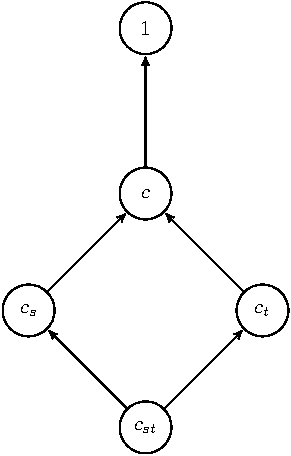
\includegraphics{hyps.pdf}
  \caption{This hierarchy of hypotheses suggests the order in which the discussed models should be tested.  One begins with the most complex models at the bottom and sequentially, following the arrows, tests simpler hypotheses using the formal test described in Section~\ref{sec:test} until a final model is established.}
  \label{fig:hier}
\end{figure}

Because the five hypotheses are nested, a natural testing order is suggested in Figure~\ref{fig:hier}.  For instance, suppose interest lies in the predator's dietary preferences with respect to prey species $s_1,s_2$ across $3$ time periods.  If it is believed that hypothesis $4.$ best describes the predator's eating, i.e.\ that the prey species are equally preferred, such that $s_1,s_2$ can be thought of as one prey, but that this preference changes across time, then 

\begin{align*}
  H_0&: \lambda_t = c_t \gamma_t, \forall t \\  
  H_1&: \lambda_{st} = c_{st}\gamma_{st}
\end{align*}

would test, statistically, if the data provide evidence for such a belief beyond the model that treats each prey species $s_1$ and $s_2$ individually across the $3$ time points.  Similarly, 

\begin{align*}
  H_0&: \lambda_s = c_s \gamma_s, \forall s \\  
  H_1&: \lambda_{st} = c_{st}\gamma_{st}
\end{align*}

would test if $P$'s eating varies by prey species, but not by time, against the most parameter rich model $c_{st}$.  The above two tests should be performed before any of the simpler methods are tested.

\subsection{Fully Observed Count Data}
\label{sec:count}

The likelihood function that allows for estimation of these parameters is as follows.  Since we assume $X_{jst}$ is independent of $Y_{ist}$ we can simply multiply the respective Poisson probability density functions, and then form products over all $s,t$ to obtain the likelihood

\begin{equation}
  \label{eq:likelihood}
 L( \boldsymbol{\lambda}, \boldsymbol{\gamma} | x_{jst}, y_{ist}) = \prod_{t = 1}^{T} \prod_{s=1}^S \left\{ \prod_{j=1}^{J_t} f_X(x_{jst}|\boldsymbol{\lambda}) \prod_{i=1}^{I_t} f_Y(y_{ist} | \boldsymbol{\gamma}) \right\}.
\end{equation}

\noindent Writing all five hypotheses as $\lambda_{st} = c_{st}\gamma_{st}$, we can, in the simplest cases, find analytic solutions for the maximum likelihood estimates (MLEs) of $c_{st}$, $\gamma_{st}$, and by invariance $\lambda_{st}$.  Such solutions exist for the simplest model, $c_{st}=1$, for which only $\gamma_{st}$ need be estimated, and for the second simplest model, $c_{st}=c$, provided that the data are balanced so that $J_t=J$ and $I_t=I$.  Respectively, these solutions are

\begin{equation*}
  \hat{\gamma}_{st} = \frac{X_{\cdot st} + Y_{\cdot st}}{J_t + I_t}, \quad \text{ and } \quad \hat{c} = \frac{I \sum_{s,t} X_{\cdot st}}{J \sum_{s,t} Y_{\cdot st}}, \quad \hat{\gamma}_{st} = \frac{X_{\cdot st} + Y_{\cdot st}}{I \left( \frac{\sum_{st} X_{\cdot st}}{\sum_{st} Y_{\cdot st}} + 1 \right)},
\end{equation*}

\noindent where $X_{\cdot st} = \sum_{j=1}^{J_t}X_{jst}$ and $Y_{\cdot st} = \sum_{i=1}^{I_t} Y_{ist}$.

In all other cases, analytic solutions are not readily available and instead we rely on the fact that the log-likelihood $l(\boldsymbol{\lambda}, \boldsymbol{\gamma}) = \log{L}$ is concave to maximise the likelihood numerically.  To compute MLEs, we maximise the log-likelihood, using coordinate descent \citep{Luo:1992}, by iteratively solving the likelihood equations (i.e.\, the equations obtained by setting the partial derivatives of the likelihood with respect to the parameters equal to zero).  This yields the following equations for updating $c$ in the models $c$, $c_t$, and $c_s$ respectively

\begin{equation*}
  \hat{c} = \frac{\sum_{s,t} X_{\cdot st}}{\sum_t J_t \sum_s \gamma_{st}}, \quad \hat{c}_t =  \frac{\sum_s X_{\cdot st}}{J_t \sum_s \gamma_{st}}, \quad \hat{c}_s = \frac{\sum_{t}X_{\cdot st}}{\sum_t J_t \gamma_{st}}, \quad \text{ and } \quad \hat{c}_{st} = \frac{X_{\cdot st}}{J_t \gamma_{st}}.
\end{equation*}

\noindent The equation for updating $\hat \gamma_{st}$ is

\[ \hat{\gamma}_{st} = \frac{X_{\cdot st} + Y_{\cdot st}}{J_t c_{st} + I_t}, \]

\noindent where $c_{st}$ would be replaced by $c, c_t$, or $c_s$ depending on the chosen model.

\subsection{Unobserved Counts}
\label{sec:noncount}

In many applications, such as DNA-based gut-content analysis, it is not possible to count the number of individuals of each prey species that are in a predator's gut.  Instead, it is only possible to detect whether or not a predator consumed the prey species during a given time period, based on the rate at which prey DNA decays in the predator gut \citep{Greenstone:2013}.  In this case we can still make inference about the predators' preferences for the different prey species by using the expectation-maximisation (EM) algorithm to compute MLEs.

We denote the binary random variable indicating whether the $j^{th}$ predator did in fact eat at least one individual of prey species $s$ in time period $t$ by $Z_{jst} = 1(X_{jst} > 0)$.  Given the Poisson assumptions above, these variables are independent Bernoulli observations with success probability $p_{st} = P(Z_{jst}=1)= 1-\exp\{-\lambda_{st}\}$.  Despite not observing $X_{jst}$, we can compute maximum likelihood estimates of the parameters $\boldsymbol{\lambda}, \boldsymbol{\gamma}$ through the EM algorithm using the complete data log-likelihood
\[
l_{comp}(\boldsymbol{\lambda}, \boldsymbol{\gamma}) = \log f_{X,Y,Z}(\boldsymbol x, \boldsymbol y, \boldsymbol z|\boldsymbol{\lambda}, \boldsymbol{\gamma}) = \sum_{s,t}^{S,T} \left[ \sum_{j=1}^{J_t} \log f_{X,Z}(x_{jst},z_{jst}|\boldsymbol{\lambda}) + \sum_{i=1}^{I_t}\log f_Y(y_{jst}|\boldsymbol{\gamma}) \right].
\]

The density of $Y_{jst}$ is exactly as in Section~\ref{sec:count} and so we focus on deriving the joint density of $X_{jst}$ and $Z_{jst}$.  With the distribution of $Z_{jst}$ given above, we can compute $f_{X,Z}(x_{jst},z_{jst}|\boldsymbol{\lambda})$ by noting that $X_{jst}=0$ with probability 1 if $Z_{jst}=0$, and that $[X_{jst}|Z_{jst}=0]$ has a truncated Poisson distribution with density
\[
  f_{X|Y,Z,\boldsymbol{\lambda},\boldsymbol{\gamma}}(x_{jst}|z_{jst}) =
  \frac{\exp{\{-\lambda_{st}\}} \lambda_{st}^{x_{jst}}}{(1 - \exp{\{-\lambda_{st}\}}) x_{jst}!}1(x_{jst} > 0)
\]
and expected value
\[
\E_{X|Y,Z}X_{jst} = \frac{\lambda_{st} \exp{\{\lambda_{st} \}}}{\exp{\{ \lambda_{st} \}} - 1}.
\]
\noindent The joint density of $X_{jst}, Z_{jst}$ is then 
\begin{equation*}
    f_{X,Z|\boldsymbol{\lambda}}(x_{jst},z_{jst}) = \left\{
    \begin{array}{lr}
      \exp{\{ -\lambda_{st} \}}, & x_{jst}=0 \mbox{ and } z_{jst} = 0 \\
      \frac{\exp{\{-\lambda_{st} \}} \lambda_{st}^{x_{jst}}}{x_{jst}!}, & x_{jst} > 0 \mbox{ and } z_{jst} = 1 \\
      0 & \mbox{otherwise}
    \end{array}
  \right..
\end{equation*}

The EM algorithm works by iterating two steps, the E-step and M-step, until the optimum is reached \citep{Dempster:1977,McLachlan:2007}.  Let $k$ index the iterations in the EM algorithm so that $\boldsymbol \lambda^{(k)}$ and $\boldsymbol \gamma^{(k)}$ denote the estimates computed on the $k^{th}$ M-step. The E-step consists of computing the expectation of $l_{comp}$ with respect to the conditional distribution of $X$ given the current estimates of the parameters
\[
Q^{(k)}(\boldsymbol{\lambda},\boldsymbol{\gamma}) = \E_{X|Y,Z,\boldsymbol{\lambda}^{(k)}} l_{comp}
\]
in order to remove the unobserved data. The M-step then involves maximising $Q^{(k)}(\boldsymbol{\lambda},\boldsymbol{\gamma})$ with respect to the parameters in the model to obtain updated estimates of the parameters,
\[
(\boldsymbol{\lambda}^{(k+1)}, \boldsymbol{\gamma}^{(k+1)}) = \argmax_{(\boldsymbol{\lambda}, \boldsymbol{\gamma})} Q^{(k)}(\boldsymbol{\lambda}, \boldsymbol{\gamma}).
\]
These steps are alternated until a convergence criterion monitoring subsequent differences in the parameter estimates/likelihood is met.  

The calculation of $Q^{(k)}(\boldsymbol{\lambda}, \boldsymbol{\gamma})$ is not difficult and is given by:
\begin{align}
  \label{eq:estep}
  \begin{split}
  Q^{(k)}(\boldsymbol{\lambda}, \boldsymbol{\gamma})
  & = \E \log{f_{X,Z|\boldsymbol{\lambda}}(X_{jst},z_{jst})} + \log{f_{Y|\boldsymbol{\gamma}}(y_{ist})} \\
  & = \sum_{s=1}^S \sum_{t=1}^T \sum_{j=1}^{J_t} \E \log{f_{X,Z|\boldsymbol{\lambda}}(X_{jst},z_{jst})}
  + \sum_{s=1}^S \sum_{t=1}^T \sum_{i=1}^{I_t} \log{f_{Y|\boldsymbol{\gamma}}(y)} \\
  & \propto \sum_{s,t,j} \left( - \lambda_{st} 
    + z_{jst} \log{\lambda_{st}} \E X_{jst} \right) + \sum_{s,t} \left( -I_t \gamma_{st} + Y_{\cdot st} \log{I_t \gamma_{st}} \right) \\
  & \propto \sum_{s,t} \left( -J_t \lambda_{st} + z_{\cdot st} \log{\lambda_{st}} \E (X_{jst}|\lambda_{st}^{(k)},\gamma_{st}^{(k)}) \right) + \sum_{s,t} \left( -I_t \gamma_{st} + Y_{\cdot st} \log{I_t \gamma_{st}} \right).
\end{split}
\end{align}
\noindent No analytic solution to the M-step exists, however, so we again chose to maximise $Q$ with coordinate descent \citep{Luo:1992}.  In fact, as we only need to find parameters that increase the value of $Q$ on each iteration, we forgo fully iterating the coordinate descent algorithm to find the maximum and instead perform just one step uphill within each EM iteration \citep{Givens:2012}.  Since $Q^{(k)}$ is concave and smooth in the parameters $\boldsymbol{\lambda}, \boldsymbol{\gamma}$, we are able to use the convergence of parameter estimates, $||(\boldsymbol{\lambda}^{(k)}, \boldsymbol{\gamma}^{(k)}) - (\boldsymbol{\lambda}^{(k+1)}, \boldsymbol{\gamma}^{(k+1)})||_{\infty} < \tau $, for some $\tau>0$, as our stopping criterion.

As we show in our simulation study, this generalised EM algorithm accurately estimates the parameters when values of $\lambda_{st}$ are relatively small, such that zeros are prevalent in the data $Z_{jst}$.  In contrast, if the predator consistently eats a given prey species, few to no zeros will show up in the observed data and $\E Z_{jst}$ is estimated to be nearly $1$.  The loss of information is best seen by attempting to solve for $\lambda_{st}$ in the equation $1 = \E Z_{jst} = 1 - \exp\{-\lambda_{st}\}$.  As the proportion of ones in the observed data increases, we expect $\lambda_{st}$ to grow exponentially large.  When no zeros are present in the data, so that only ones are observed, the likelihood can be made arbitrarily large by sending the parameter off to infinity.  

\subsection{Testing}
\label{sec:test}
The likelihood ratio test statistic is

\begin{equation*}
  \label{eq:LRT}
    \Lambda(X,Y) := -2 \log{ \frac{ \sup_{\theta_0} L(\theta_0|X,Y)}{ \sup_{\theta_1} L(\theta_1|X,Y)} },
\end{equation*}

\noindent where $\theta_0, \theta_1$ represent the parameters estimated under the null and alternative hypotheses, respectively.  It is well known that the asymptotic distribution of $\Lambda$ is a $\chi_{\rho}^2$ distribution with $\rho$ degrees of freedom \citep{Wilks:1938}.  The degrees of freedom $\rho$ equal the number of free parameters available in the stated hypotheses under question.  If we put the null hypothesis to be $H_0: \lambda_t = c_t \gamma_t$, for all $t$ and contrast this against $H_1: \lambda_{st} = c_{st}\gamma_{st}$ then there are $\rho = 2(S \cdot T) - S \cdot T - T = S \cdot T - T$ degrees of freedom.  When the observations $X_{jst}$ are not observed, we use $L_{obs}(\boldsymbol{\lambda}, \boldsymbol{\gamma}|Z,Y)$ as the likelihood in the calculation of $\Lambda$

\[ L_{obs}(\boldsymbol{\lambda}, \boldsymbol{\gamma}|Z,Y) = \prod_{s,t}^{S,T} \left\{ \prod_{j=1}^{J_t}f_Z(z_{jst}|\boldsymbol{\lambda}) \prod_{i=1}^{I_t}f_Y(y_{ist}|\boldsymbol{\gamma}) \right\}. \]

\noindent The level of significance $\alpha$ is used to reject the null hypothesis in favour of the alternative hypothesis if $\mathbb{P}(\chi^2_{\rho} > \Lambda) < \alpha$.  

\subsection{Linear Transformations of $c_{st}$}

After determining which model best fits the data, more detail may be extracted through specific hypothesis test of the elements of $c_{st}$, or in vector notation as $\mathbf{c} \in \mathbb{R}^{S\cdot T}$.  Let the elements of $\hat{\mathbf{c}}$ be the maximum likelihood estimates, $\hat{c}_{st}$, as found via the framework above.  Since $\hat{\mathbf{c}}$ is asymptotically normally distributed, any linear combination of the elements is also asymptotically normally distributed.  For instance, let $a$ be a vector of the same dimension of $\hat{\mathbf{c}}$.  Then $a^t\hat{\mathbf{c}}$ is asymptotically distributed as $\mathcal{N}(a^t\mathbf{c}, a^t\Sigma a)$, where $\Sigma$ is the covariance matrix of the asymptotic distribution of $\hat{\mathbf{c}}$.  Tests of the form $H_0: a^t\mathbf{c} = \mu$ against any alternative of interest are then approximate $Z$-tests.  Confidence intervals of any size are similarly, readily obtained.  Suppose, for example, that the hypothesis $c_s$ is determined to best fit the data with $s$ ranging $s = 1, 2, 3$.  We can test to see whether or not the first two species are equally preferred under the null hypothesis $c_{1} = c_{2}$.  This hypothesis is alternatively written in vector notation as $a^t\mathbf{c} = 0$, where $a = (1, -1, 0)^t$.  

\section{Simulation Study}
\label{sec:sim}

Our simulations assume two prey species and five time points, throughout.  Of the hierarchy of hypotheses, we generate data under three models: $c, c_s, c_t$.  Sample sizes for both prey species and predator gut count observations are randomly chosen from four overlapping levels: ``small'' sample sizes are randomly sampled numbers in $[20,50]$, ``medium'' $[30,75]$, ``large'' $[50,150]$, and ``larger'' $[100,200]$.  This is repeated for each level of sample size.  We simulate $500$ replicate data sets for each of the twelve scenarios above for both types of data, fully observed count data, $X_{jst}$, and for non-count data, when we observe only a binary response, $Z_{jst} = 1(X_{jst}>0)$.  Each scenario is then fitted with the true model that generated the data.  All simulations of non-count data use $\tau = 10^{-5}$ as the convergence tolerance.  A subset of the examples are provided here; the interested reader is referred to the supplementary materials for the complete simulation results.

\begin{figure}
  \textbf{Small Sample Size}\par
  \centering
  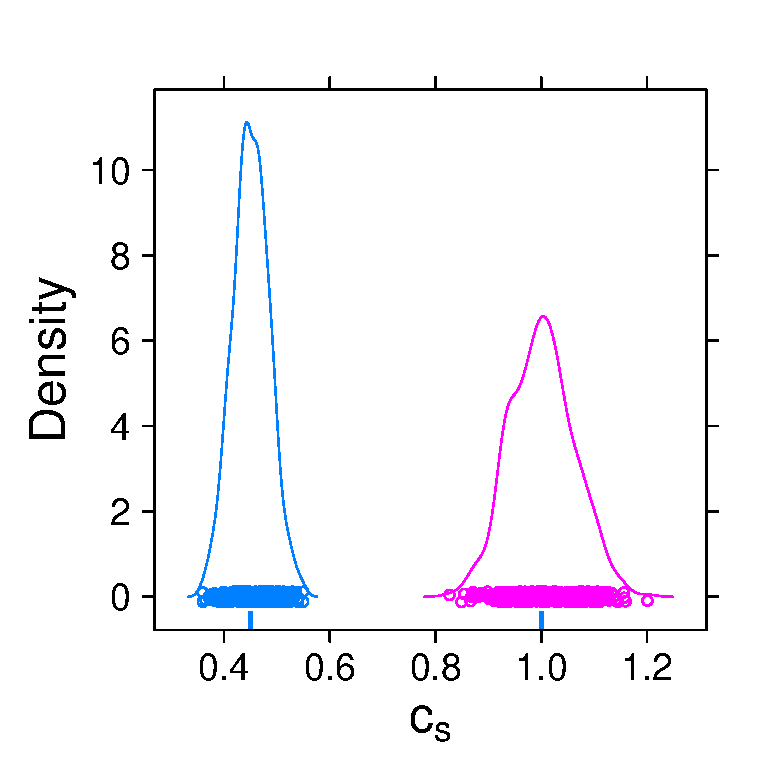
\includegraphics[scale=0.75]{small}
  \caption{The density plot of all $500$ estimates of fitting the true model to the data generated from models $c_s$ with the small sample size is shown.  Each element of $c_s$ is colour coded for clarity, and ticks on the x-axis show the true parameter values.}
  \label{fig:small}
\end{figure}

For all simulated data, the true parameter values for the rate at which prey species are encountered in the wild are fixed to be $\gamma_{st} = \pi \approx 3.14, \, \forall s,t$.  The values of $\lambda_{st}$ are set with respect to each data generating model.  For model $c_{st} = c$, where predator preferences don't vary by either time or species, we put $\lambda_{st} = 2\pi, \forall s,t$.  Under model $c_s$, the ratio of rates vary by species only, so we put $\lambda_{1t} = \sqrt{2}$ and $\lambda_{2t} = \pi$.  Hence, $c_1 = \sqrt{2}/\pi \approx 0.45$ and $c_2 = 1$.  For the last model, $c_t$, the ratio of rates vary by time $t$.  Here, we put $\lambda_{st} = t$ for $t \in \{1, \ldots, 5 \}$.  

\begin{figure}
  \textbf{Medium Sample Size}\par
  \centering
  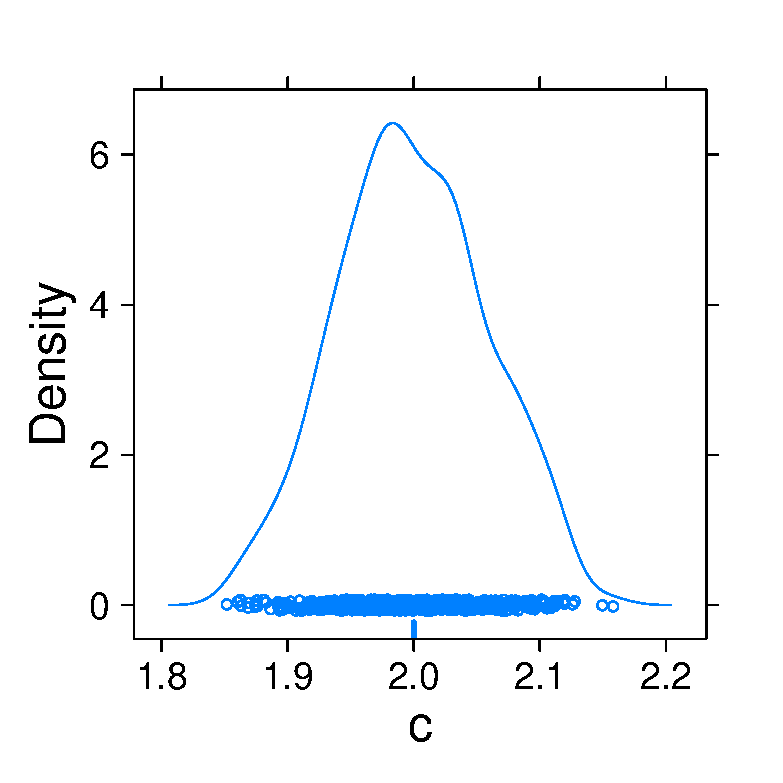
\includegraphics[scale=0.75]{medium}
  \caption{The density plot of all $500$ estimates of fitting the true model to the data generated from model $c$ with the medium sample size is shown.  A tick on the x-axis shows the true parameter value.}
  \label{fig:medium}
\end{figure}

We consider results when the correct model is fit to the simulated data.  Figure~\ref{fig:small} shows the density plot of the estimates of $c_s$ when fitting the true model to the fully observed count data generated under models $c_s$, while Figure~\ref{fig:medium} shows the same for the estimates of $c$ when data is generated under model $c$.  The plots provide evaluations of parameter estimates under each scenario.  For model $c_s$ in Figure~\ref{fig:small}, the parameters $c_1 \approx 0.45$ and $c_2 = 1$ are on average, across all $500$ simulations, estimated as $\hat{c}_1 = 0.45$ and $\hat{c}_2 = 1.00$, with sample standard deviations of $\text{SD}(\hat{c}_1) = 0.03$ and $\text{SD}(\hat{c}_2) = 0.06$.  Figure~\ref{fig:medium} provides results for model $c_{st} = c$.  Averaging across all $500$ simulations, the parameter $c=2$ is estimated as $\hat{c} = 2.00$ with sample standard deviation $\text{SD}(\hat{c})=0.06$.  This is further seen in Figure~\ref{fig:bp}, where box plots of the parameter estimates, centred at true parameter values, of the correct model fit to data generated from both $c_s$ and $c_t$ show empirically very little bias.

\begin{figure}
  \centering
  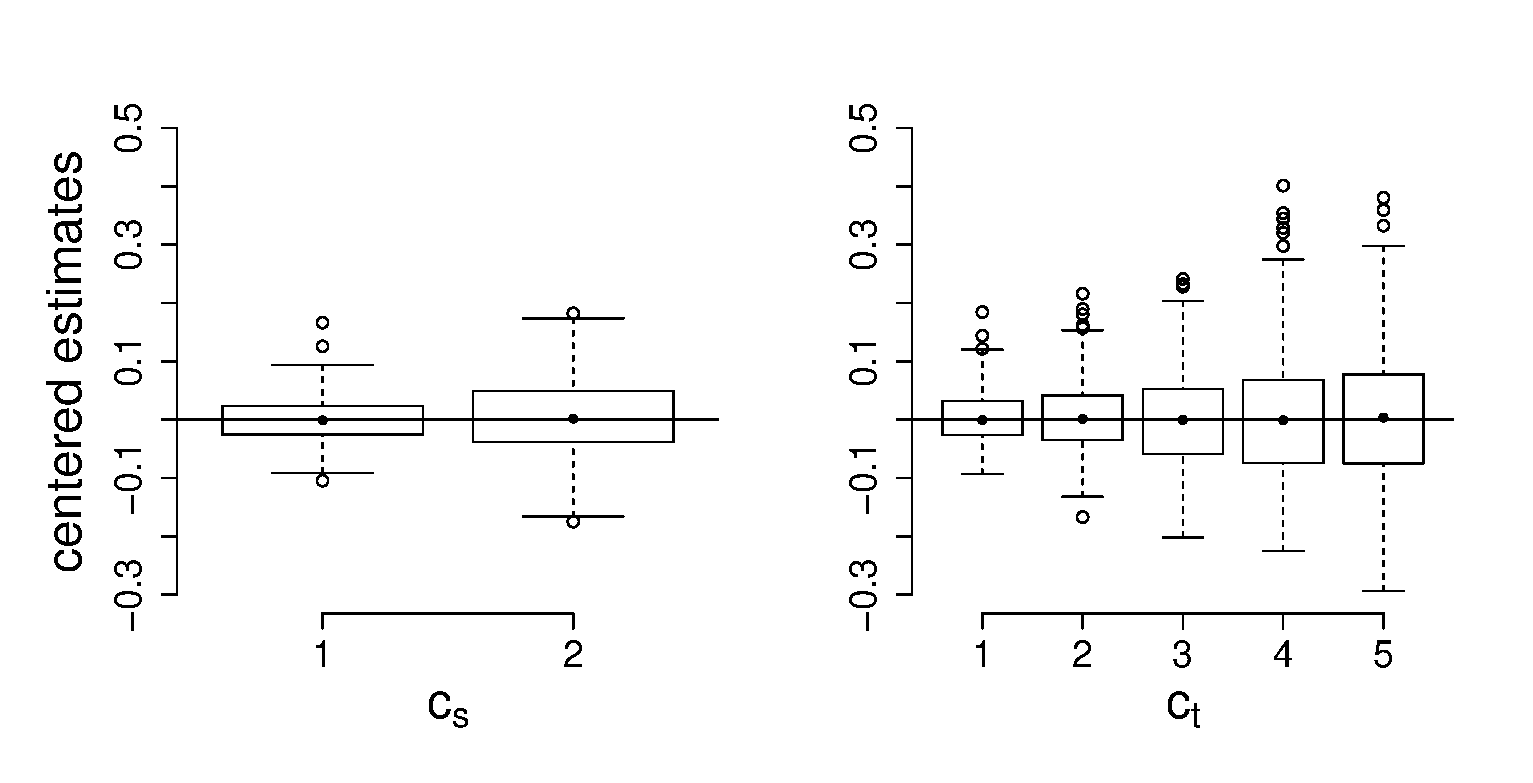
\includegraphics[scale=0.5]{bp}
  \caption{Shown are all $500$ estimates, cent-red at the true parameter values, from fitting the true model to the data generated from models $c_s,c_t$ with sample sizes small and medium, respectively.}
  \label{fig:bp}
\end{figure}

We next generated data with unobserved counts.  As noted above under certain circumstances our unobserved counts model accurately estimates the parameters of interest, and at other times can infinitely over-estimate parameters.  To investigate this issue further, we consider the same scenarios mentioned above, but reduce all of the count data down to binary observations.  For each scenario, we fit the unobserved counts model as if we knew the true underlying model that generated the observed data.

Figures \ref{fig:smallEM} and \ref{fig:largerEM} contain density plots of the estimates of $c_s, c_t$ for all $500$ replications of the data generating models $c_s,c_t$ with the small and the larger sample sizes, respectively.  When data are generated under the model $c_s$ and the true model is fit to the non-count data, we find even for the small sample size that point estimates are only very slightly biased.  When parameter values are of sufficient size to make zeros in the simulated data less common, the estimates from fitting the correct model to the generated data are occasionally over-estimated.  This effect is easily seen in Figure~\ref{fig:largerEM} for the two greatest values of $c_t$ despite the increased sample size, but is also seen, less dramatically, in the density plot for the $c_s$ generated data.  

\begin{figure}
  \textbf{Small Sample Size, Non-Count Data}\par
  \centering
  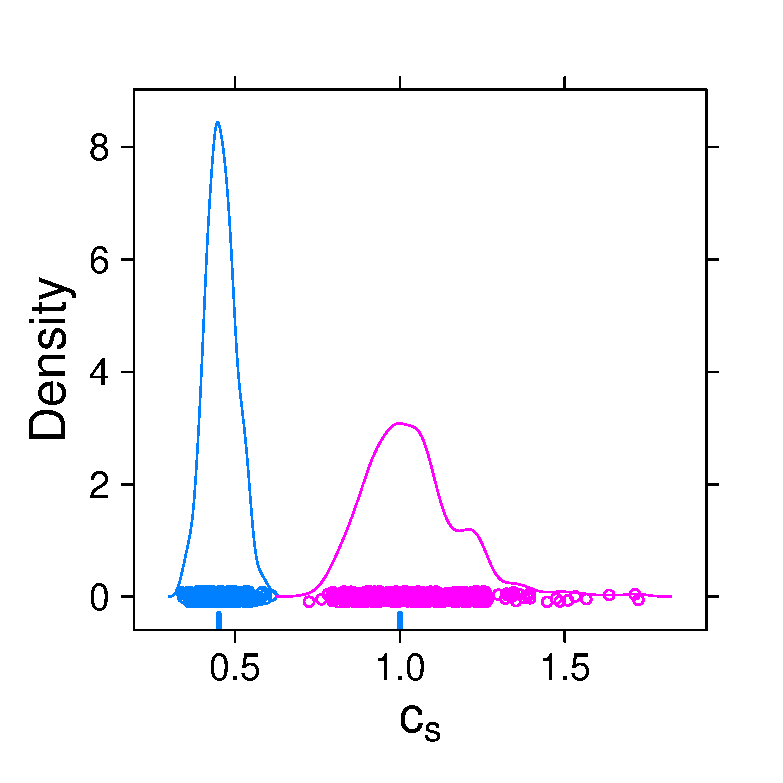
\includegraphics[scale=0.75]{smallEM}
  \caption{The density plot of all $500$ estimates of fitting the true model to the data generated from model $c_s$, when counts are not observed, is shown with the small sample size.  Each element of $c_s$ is colour coded for clarity, and ticks on the x-axis show the true parameter values.}
  \label{fig:smallEM}
\end{figure}

The cluster of estimates for $c_5$ between $3.5$ and $4.0$ in Figure~\ref{fig:largerEM} comes from data sets in which $Z_{js5}=1$ for all $j,s$.  For the data shown in Figure~\ref{fig:largerEM}, this happened $73$ times out of the $500$ replicated data sets.  As mentioned above, the estimate of $c_5$ is infinite in this case.  However, the EM algorithm will always provide a finite estimate for all parameters when it terminates.  In this case, we set $\tau=10^{-5}$ and this caused the algorithm to terminate with $\hat c_5$ between $3.5$ and $4.0$.  To confirm that this is due to the arbitrary choice of $\tau$, we repeated the algorithm with smaller values of $\tau$ for several data sets. As expected, $\hat c_5$ increased without bound as we refit the model with increasingly small values of $\tau$.

\begin{figure}
  \textbf{Larger Sample Size, Non-Count Data}\par
  \centering
  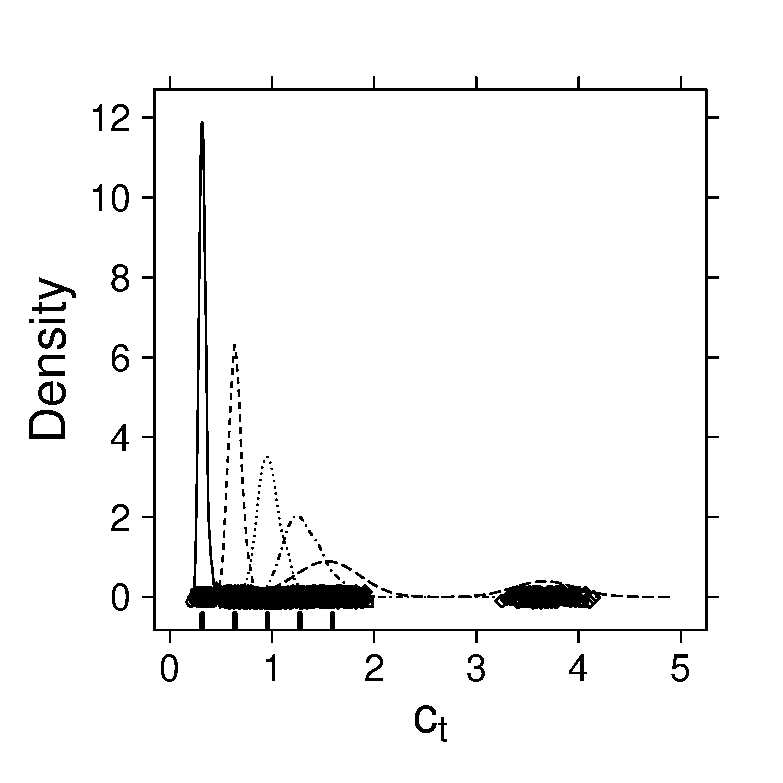
\includegraphics[scale=0.75]{largerEM}
  \caption{The density plot of all $500$ estimates of fitting the true model to the data generated from model $c_t$, when counts are not observed, is shown with the larger sample size.  Each element of $c_t$ is colour coded for clarity, and ticks on the x-axis show the true parameter values.}
  \label{fig:largerEM}
\end{figure}

The over-estimation of parameters, a symptom of the loss of information due to the unobserved counts, can also be seen with box plots of the $500$ point estimates centred at their respective true parameter values.  Figure~\ref{fig:em_bp} contains box plots of the same scenarios in Figures \ref{fig:smallEM} and \ref{fig:largerEM}.  For the $73$ cases in which $Z_{js5} = 1$ for all $j,s$ under model $c_t$ with the larger sample size, the bias is infinite since parameter estimates will, theoretically, be infinite.  The finite bias shown in these plots is due to the finite estimates provided by the termination of the EM algorithm.  Thus, conditional on a mixture of $0$s and $1$s in the data the corresponding estimators appear to be unbiased, but when no $0$s exist in the data the theoretical bias is infinite.  

\begin{figure}
  \centering
  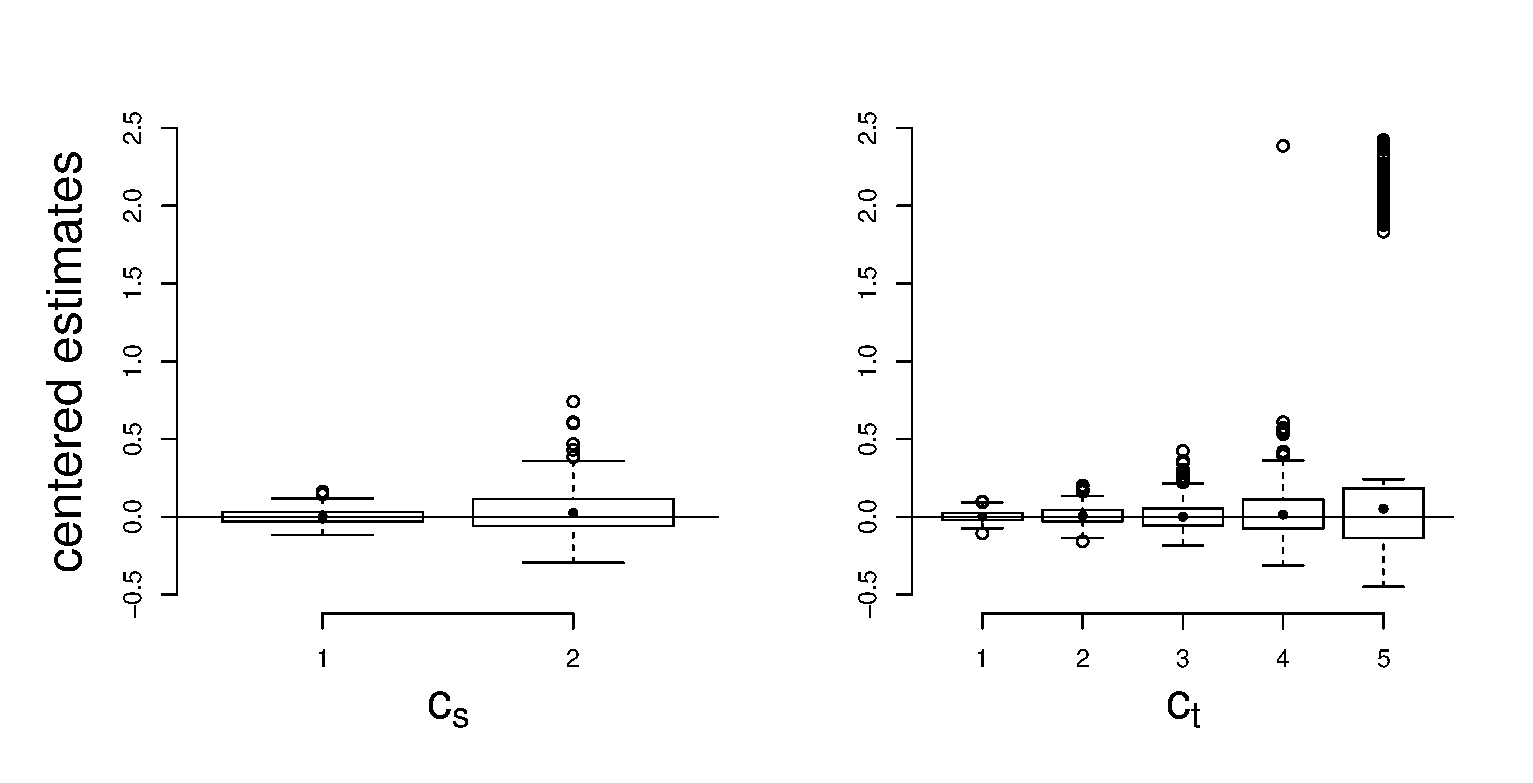
\includegraphics[scale=0.5]{em_bp}
  \caption{Shown are all $500$ estimates, centred at the true parameter values, from fitting the true model to the data generated from models $c_s,c_t$, when counts are not observed, with sample sizes small and larger, respectively.}
  \label{fig:em_bp}
\end{figure}

\section{Application}
\label{sec:data}

To illustrate these methods, we analysed a data set collected to investigate the feeding preferences of two species of wolf spider, Schizocosa ocreata and Schizocosa stridulans (Araneae: Lycosidae).  Every $6-12$ days, $10$ to $40$ spiders were hand-collected between October $2011$ and April $2013$ within Berea College Forest in Madison County, Kentucky, USA.  Spiders were removed from the leaf litter using an aspirator, placed in separate $1.5$ mL microcentrifuge tubes filled with $95$\% EtOH, and preserved at $-20\celsius$ until DNA extraction.  In parallel, we also surveyed availability of forest floor prey using pitfall traps $(n = 32)$.  For the analysis, both species of Schizocosa were pooled and the number of spiders and prey were analysed by month.  On average, $69$ spiders, $111$ Diptera, and $297$ Collembola were caught in each time period.  The range of the sample sizes across all $18$ months was $11$ to $181$ for caught spiders, $7$ to $322$ for trapped Diptera, and $101$ to $755$ for trapped Collembola.  Figure~\ref{fig:trapped} plots the total number of each order that was caught during each time period.

\begin{table}
  \label{tab:s1}
  \centering
  \begin{tabular}{llll}
    \hline
    \textbf{Target group} & \textbf{Primer names and sequences} $5'-3'$ & \textbf{Size (bp)} & \textbf{Source}\\
    \hline
    Collembola & Col3F: GGACGATYTTRTTRGTTCGT & 228 & \citet{Sint:2012} \\
    & Col-gen-A246: TTTCACCTCTAACGTCGCAG & & \\
    Diptera & DIPS16: CACTTGCTTCTTAAATrGACAAATT & 198 & \citet{Eitzinger:2014} \\
    & DIPA17: TTyATGTGAACAGTTTCAGTyCA &  & \\
  \end{tabular}
  \caption{Targeted prey orders, primer names and sequences, size of amplicon, and source of design for the detection of prey taxa within the guts of Schizocosa spiders.  Both primer sets were used in singleplex PCR assays.}
\end{table}

To determine whether spiders had consumed dipterans and/or collemblans, we conducted a molecular analysis of their gut-contents.  First, DNA from spiders was extracted using Qiagen DNEasy\circledR Tissue Extraction Kit (Qiagen Inc., Chatsworth, California, USA) following the animal tissue protocol outlined by the manufacturer, with minor modifications.  Whole bodies of the spiders were first crushed to release prey DNA from within their alimentary canal for extraction.  The $200 \mu$L extractions were stored at $-20\celsius$ until PCR.  Second, order-specific primers from the literature were used to detect the DNA of Collembola and Diptera within the guts of the spiders.  Primer pairs designed by \citet{Sint:2012}, targeting the $18$S rDNA gene, were used to detect Collembola predation Table~\ref{tab:s1}.  A PCR cycling protocol for $12.5 \mu$L reactions containing $1x$ Takara buffer (Takara Bio Inc., Shiga, Japan), $0.2$ mM dNTPs, $0.2 \mu$M of each primer, $0.625$ U Takara Ex TaqTM and $1.5 \mu$L of template DNA, using BioRad PTC$-200$ and C$1000$ thermal cyclers (Bio-Rad Laboratories, Hercules, California, USA), was optimised as follows: $95\celsius$ for $1$ minute, followed by $35$ cycles of $94\celsius$ for $30$ seconds, $61.2\celsius$ for $90$ seconds, and $72\celsius$ for $60$ seconds.  Primer pairs designed by \citet{Eitzinger:2014}, targeting the $18$S rDNA gene, were used to detect Diptera predation Table~\ref{tab:s1}.  PCR cycling protocol for $12.5 \mu$L reactions with Takara reagents (as above) and $2 \mu$L of template DNA was optimised as follows: $95\celsius$ for $1$ minute, followed by $40$ cycles of $94$ for $45$ seconds, $60\celsius$ for $45$ seconds, and $72\celsius$ for $45$ seconds.  Both primer pairs were tested for cross-reactivity against a range of prey and predator species from the field site and in all cases, no amplification of DNA was observed, confirming suitable specificity of the primers for this study.  Lastly, electrophoresis of $10 \mu$L of each PCR product was later conducted to determine success of DNA amplification using $2\%$ Seakem agarose (Lonza, Rockland, Maine, USA) stained with $1x$ GelRed\texttrademark nucleic acid stain (Biotium, Hayward, California, USA).  This procedure allowed us to determine a presence or an absence of Diptera and Collembola DNA within each spider. 

\begin{figure}
  \centering
  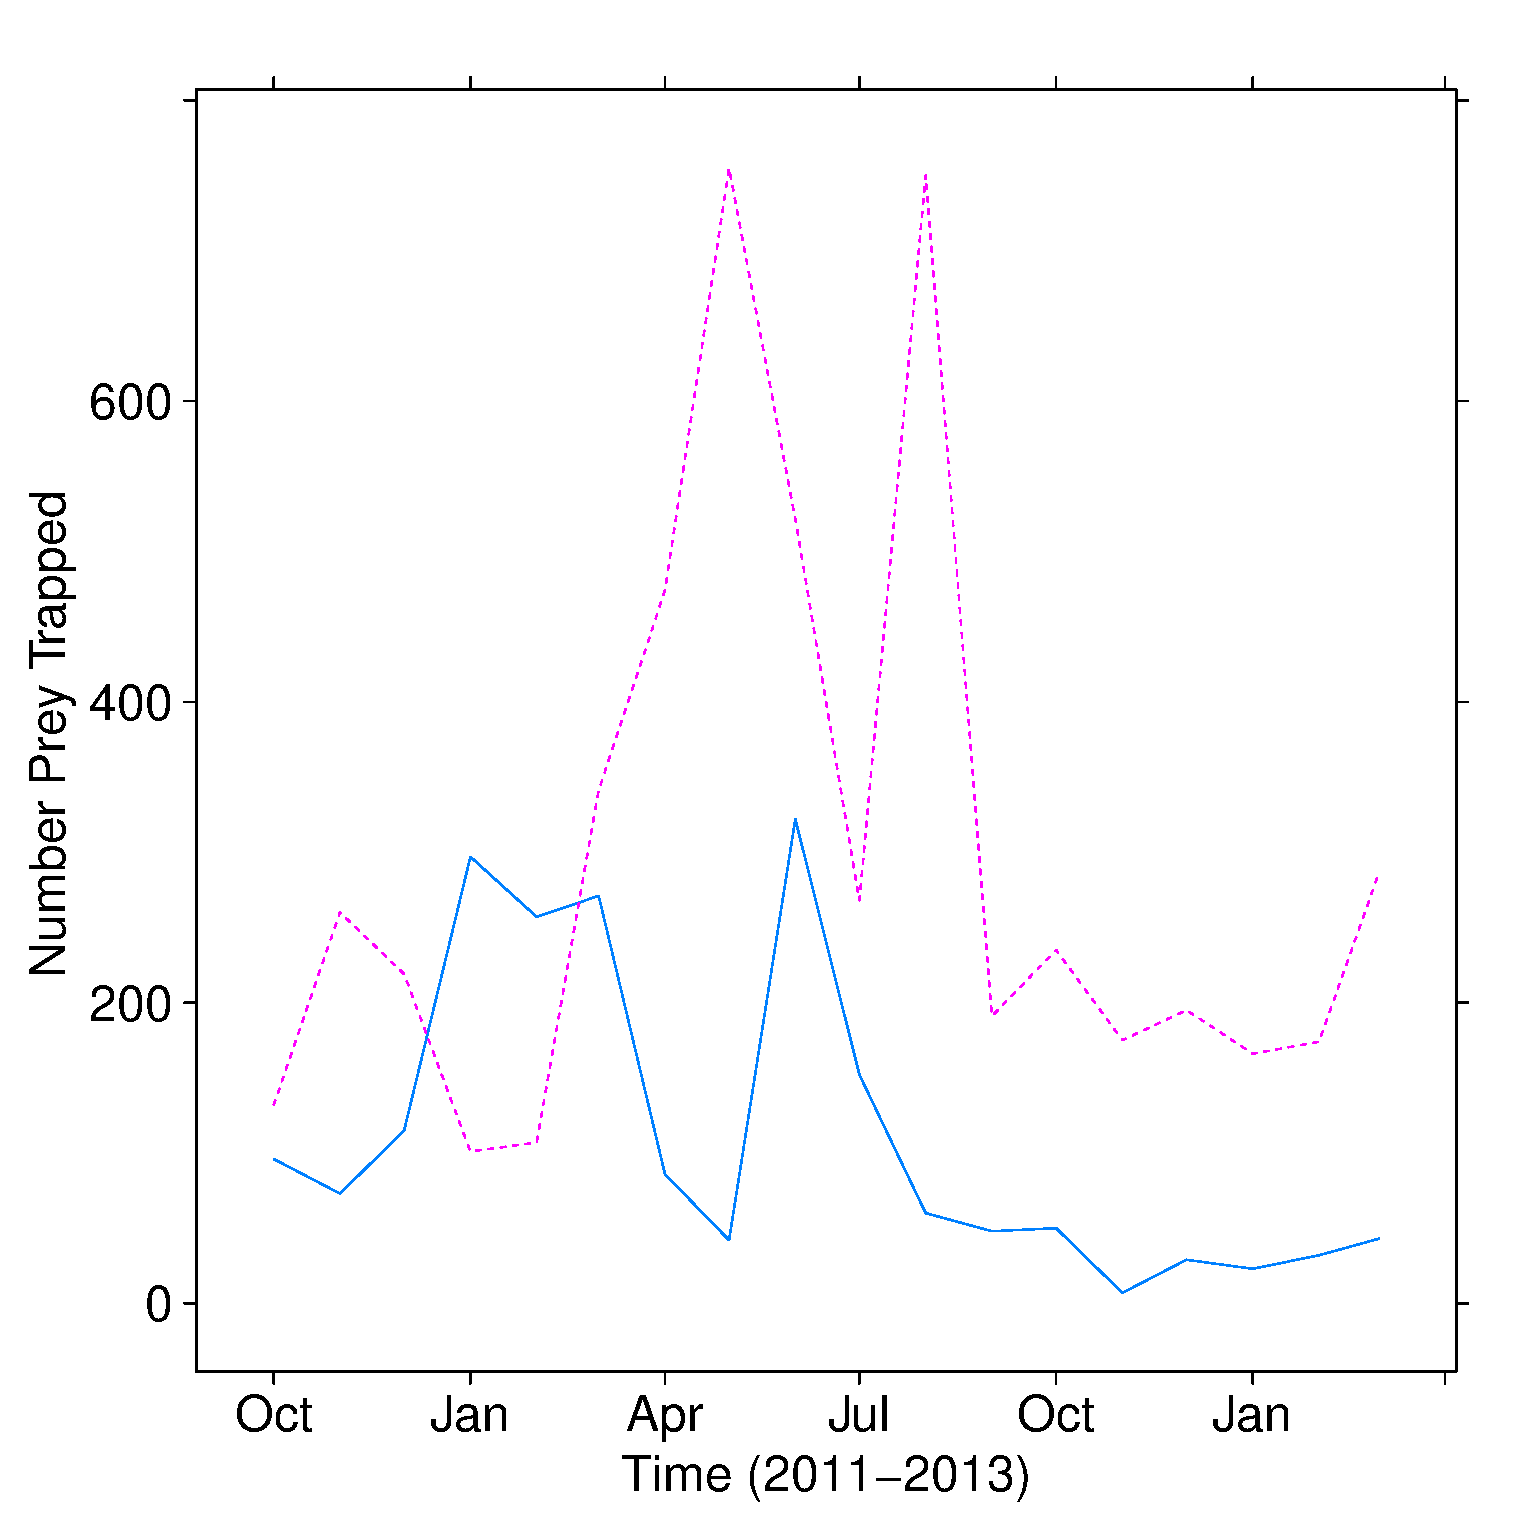
\includegraphics[scale=0.35]{prey_trapped}
  \caption{For both Collembola (pink/dashed) and Diptera (blue/solid), the plot shows the number of the prey trapped in each time period.}
  \label{fig:trapped}
\end{figure}

\begin{figure}
  \centering
  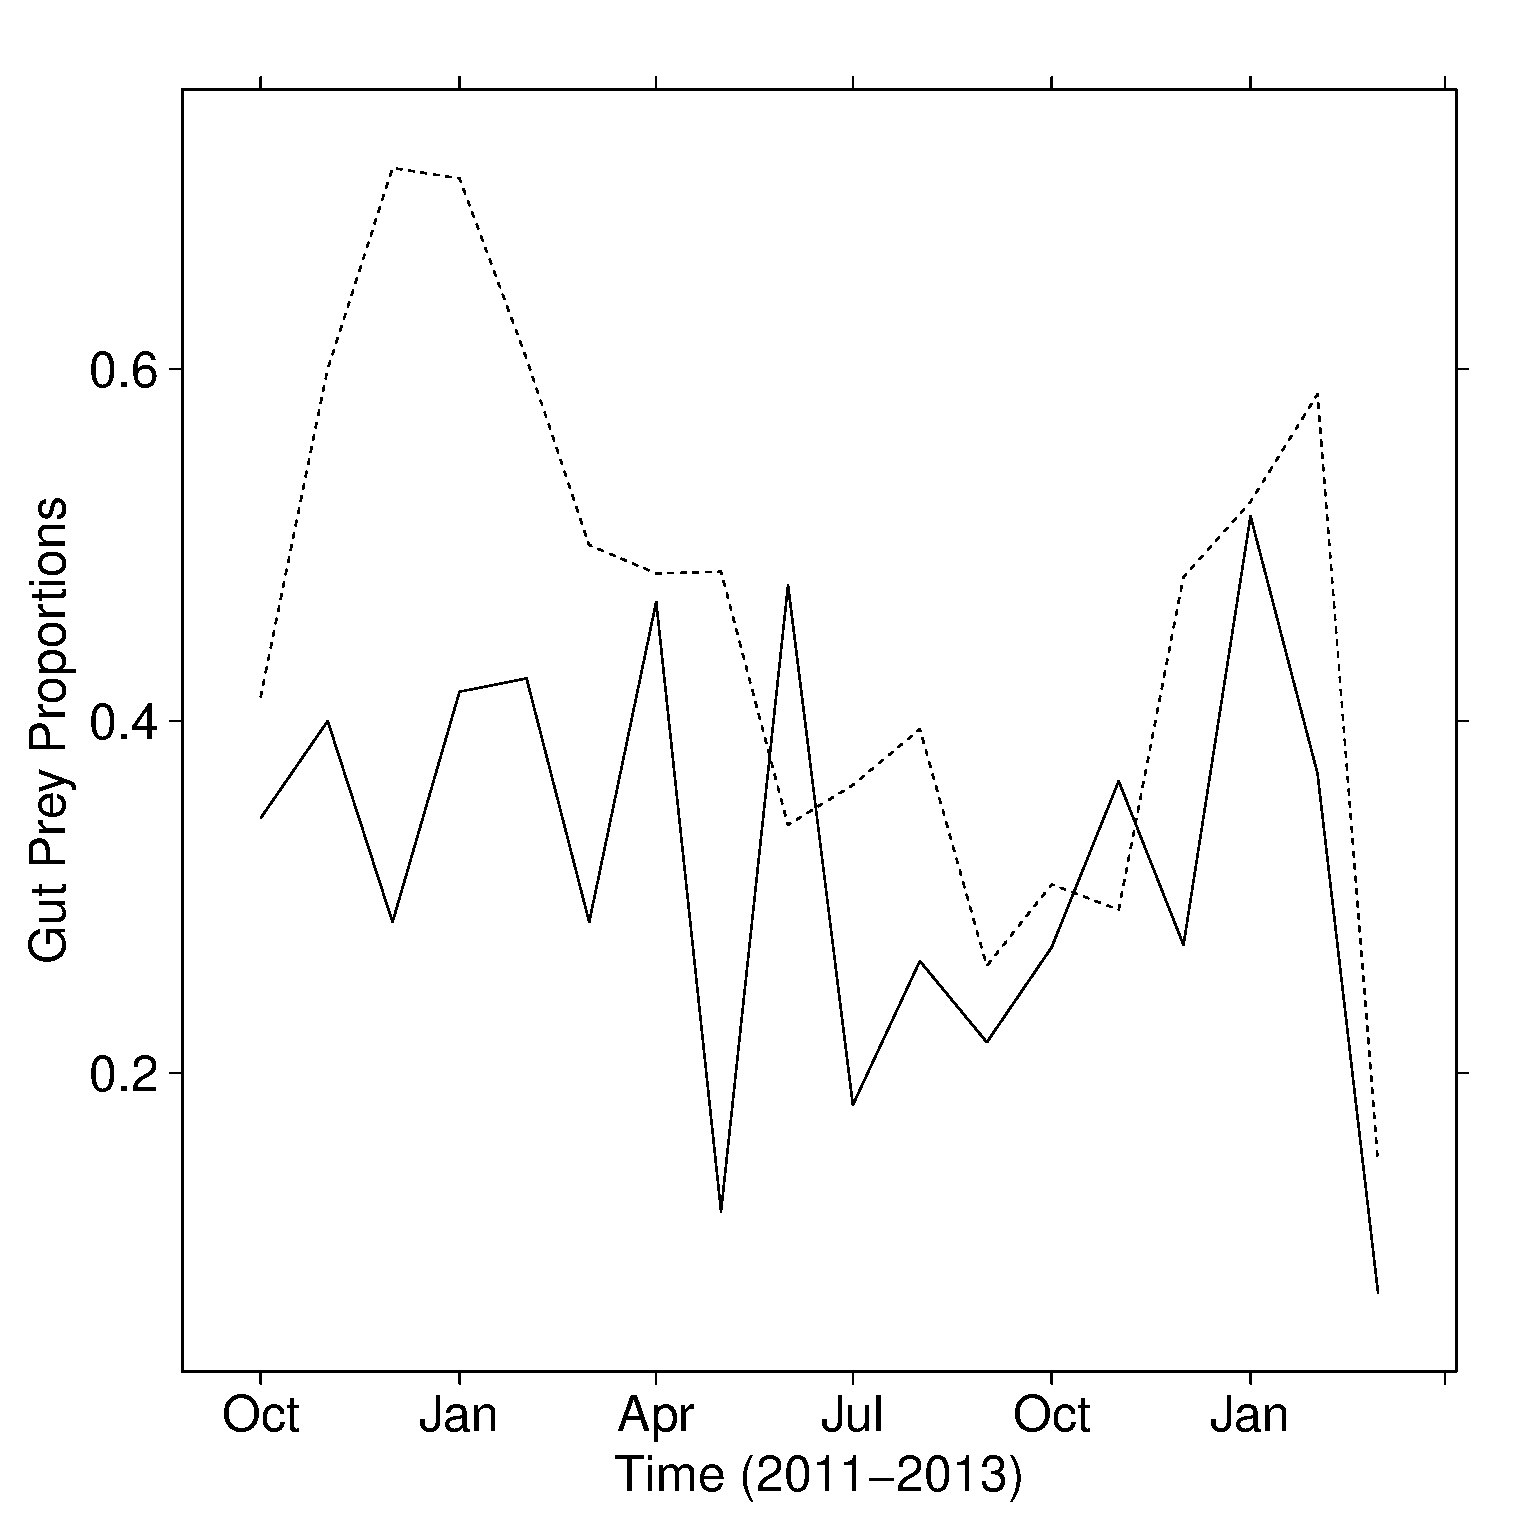
\includegraphics[scale=0.35]{prey_props}
  \caption{For both Collembola (pink/dashed) and Diptera (blue/solid), the plot shows the prey proportions in the sampled wolf spiders' guts in each time period.}
  \label{fig:props}
\end{figure}


These data provide an example of our hierarchy of hypotheses.  From the bottom of the graph in Figure~\ref{fig:hier}, we tested the most parameter rich model $c_{st} = \lambda_{st}/\gamma_{st}$ against models $c_{s}, c_{t}$.  In both cases, the more parameter rich model fits these data better than is expected by chance; $H_0: c_s$ versus $H_1: c_{st}$ gives p-value $< 0.0001$ and $H_0: c_t$ versus $H_1: c_{st}$ gives p-value $< 0.0001$.  Model $c_{st}$ estimates $72$ parameters in total; since, in this case, there are two prey of interest and $18$ time periods, it takes $36$ parameters to estimate each $c_{st}$ and $\gamma_{st}$.  Figures~\ref{fig:est_coll},~\ref{fig:est_dipt} plot the point estimates and $95\%$ confidence intervals of $c_{st}$, for both prey across all time periods.  

\begin{figure}
  \centering
  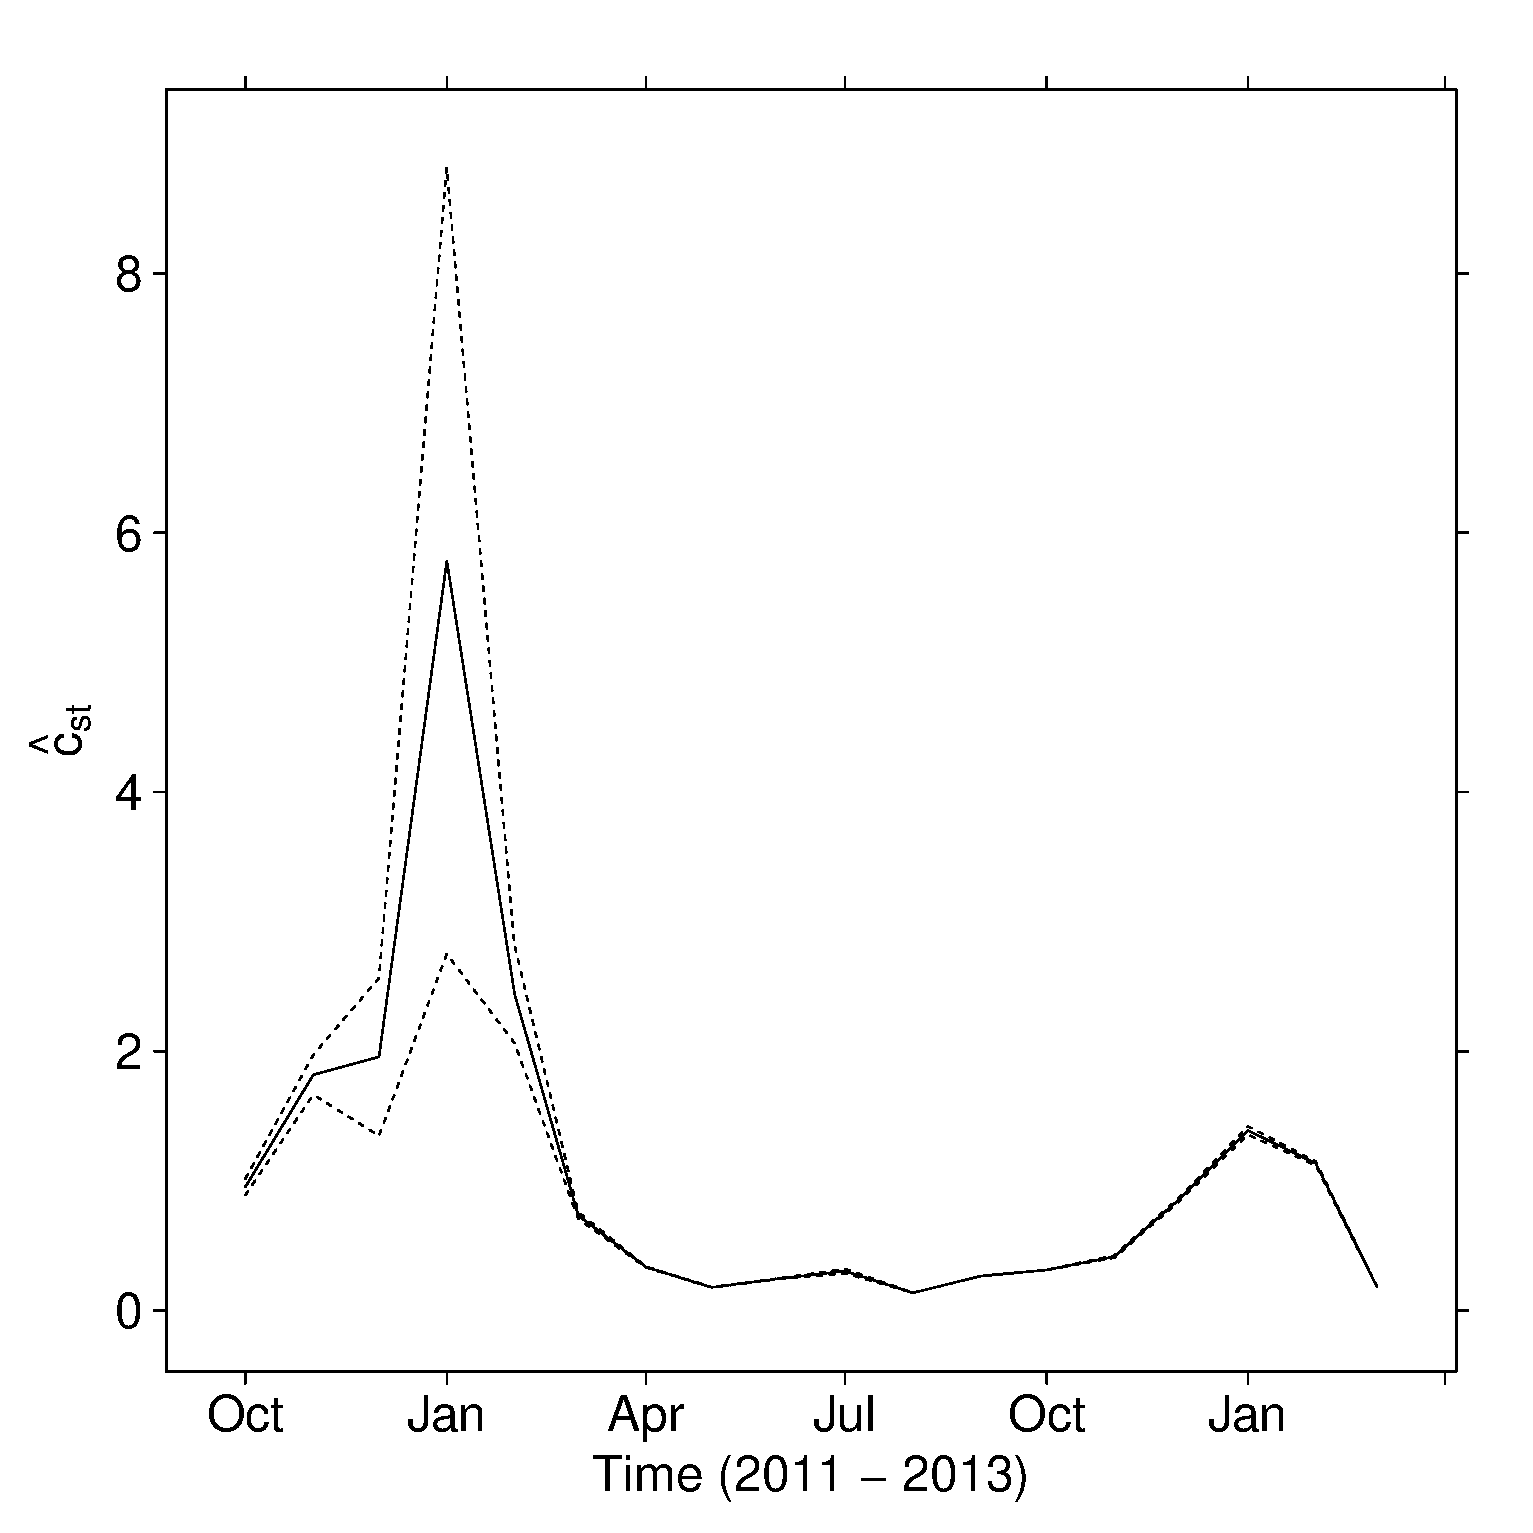
\includegraphics[scale=0.35]{est_coll}
  \caption{Point estimates (blue/solid) and $95\%$ confidence intervals (pink/dashed) as estimated from the model $c_{st}$ for Collembola.}
  \label{fig:est_coll}
\end{figure}

\begin{figure}
  \centering
  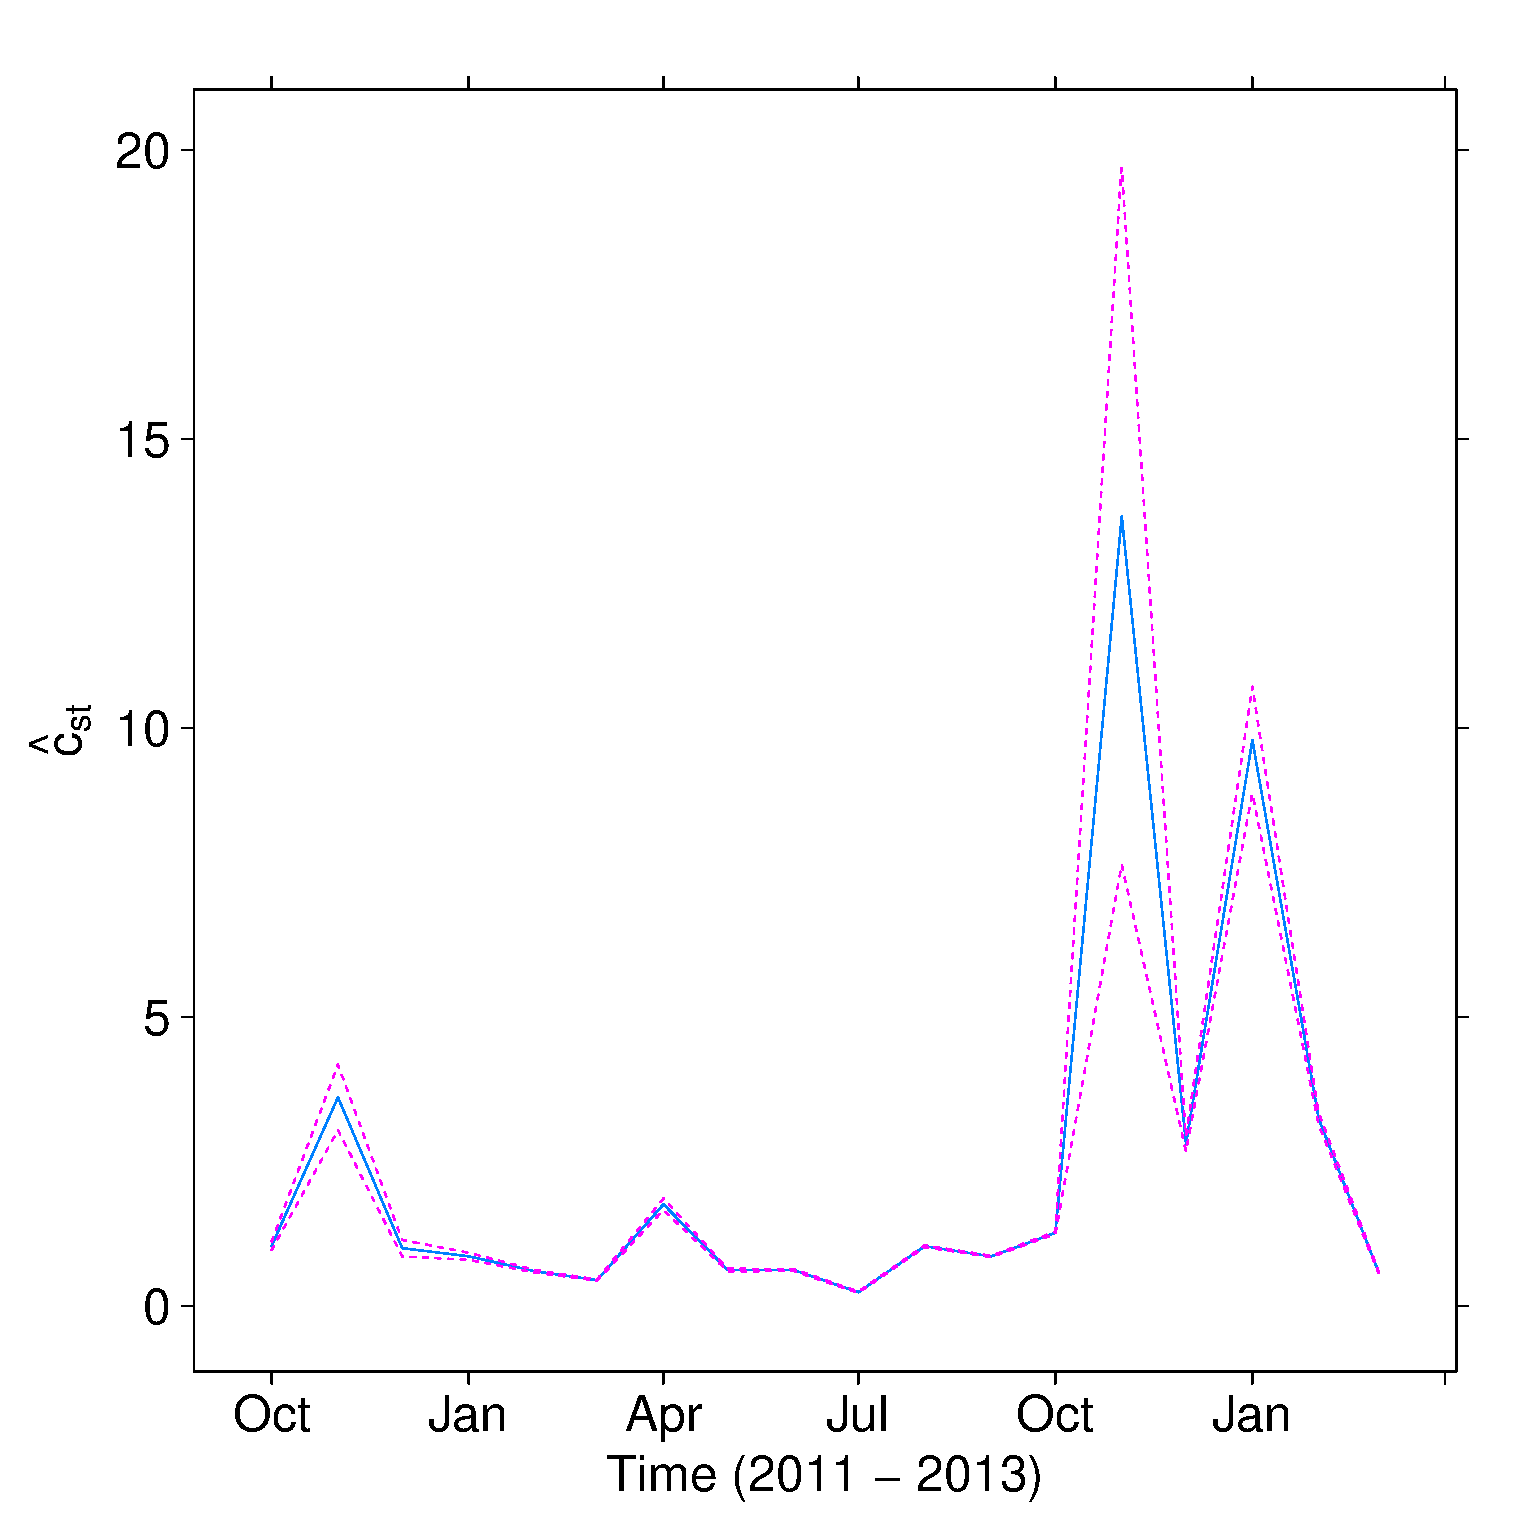
\includegraphics[scale=0.35]{est_dipt}
  \caption{Point estimates (blue/solid) and $95\%$ confidence intervals (pink/dashed) as estimated from the model $c_{st}$ for Diptera.}
  \label{fig:est_dipt}
\end{figure}

With point estimates of $c_{st}$ under the model $c_{st} = \lambda_{st}/\gamma_{st}$, we can test any number of linear contrasts.  For instance, the hypotheses $c_{1t} = c_{2t}$, for $t \in \{1, \ldots, 18\}$ state that wolf spiders equally prefer the orders Diptera and Collembola at each of the $18$ time points.  Using a level of significance of $0.05$, and after making a Bonferroni multiple comparisons adjustment, the data can not say that the two prey are differently preferred in October, November, and December of $2011$ and for March and July of $2012$.  {\color{red} What does this tell us/someone? Just a quick sentence.}

\section{Discussion}
\label{sec:discussion}

All the methods mentioned here, whether they be others' methods or our model, are susceptible to a number of issues that must be handled as best as possible by the investigator.  The most obvious are sampling issues of prey and predator species of interest.  It is almost impossible to know how well one's data represents the habitat and the availability of the prey of interest.  Variables not recorded when collecting data could have influenced the relative abundance of species that were caught.  And yet this is just the beginning.  Other practical challenges of analysing the data once in the lab provide immense opportunity for data to be comprimised.  We therefore, in this paper, focused solely on the methodologies themselves, assuming the best of possible scenarios brought your data to our model.

The earliest estimators of predators' dietary preferences, summarised by \citet{Lechowicz:1982} and \citet{Manly:2002},  produced one number summaries that rarely considered more than one prey species of interest, did not take into account changes across time, and had minimal statistical justification.  Instead, the indices developed were justified by arguing in favor of each index's unique, and claimed ``optimal,'' properties.  We feel these indices missed the point; an index is only as good as it is understood to estimate and model our world of observable data.  

A more recent and notable method to esimate predator's preferences uses a Monte Carlo, or bootstrap to be more accurate, approach \citep{Agusti:2003}.  This method deserves credit for its lack of distributional assumptions, and yet it still misses the benefits of formally modelling multiple prey species and multiple time points.  Further, it should be noted that this Monte Carlo approach though creative and widely applicable, easily confuses a key statistical idea: re-sampling does not in any way increase one's sample size or the information contained there within.

The model presented here is a formal statistical model, which enables hypothesis testing of multiple prey species across an array of time points.  When appropriately fit to data our methods, via a likelihood ratio test, offer greater statistical power than any index or distribution-free Monte Carlo methods do.  Robust simulations provided insight into the statistical properties of our model.  Moreover, we can estimate parameters of interest even when the predator's gut contents are not fully observed.  

Throughout this paper we assume the observed data were generated from Poisson distributions.  This enabled us to use the expectation-maximisation algorithm to fit our model when only incomplete data is observed.  Of course, other distributional assumptions could be made in the case of fully observed count data, but it is not clear if this is true in the case of the unobserved count data.  For instance, consider simply replacing the Poisson distribution with a distribution that has more than one parameter.  Since, in the case of non-count data only $0$s and $1$s are observed, a distribution with more than one parameter would be over-identified.  The only other option is to specify a distribution that better fits the observed data than the Poisson distribution, but here one needs to be careful about the underyling processes that are being modelled.  

{\color{red} So what does our model offer ecologists? Just a quick paragraph.}

Further developments of our model could take into account other environmental variables that might affect a predator's eating habits, such as rain or temperature.  

\begin{acknowledgements}
The information reported in this paper (No.\ $15-08-008$) is part of a project of the Kentucky Agricultural Experiment Station and is published with the approval of the Director.  Support for this research was provided by the University of Kentucky Agricultural Experiment Station State Project KY008055 and the National Science Foundation Graduate Research Fellowship Program.  
\end{acknowledgements}
% \section{Data Accessibility}
% \label{sec:accessibility}

% An \texttt{R} package, named \texttt{spiders}, is available on CRAN at \url{http://cran.r-project.org/web/packages/spiders/index.html} and fits all the methods discussed above.  \nocite{Wickham:2011a,Wickham:2011,Bischl:2014}

\bibliographystyle{spbasic}
\bibliography{refs}
\end{document}

%%% Local Variables:
%%% mode: latex
%%% TeX-master: t
%%% End:
